\chapter{Theory and Goals}
The image recognition im going to make is animal recognition. It is a simple project but can truly showcase the abilities of model, the affects of the training and how good the results are.

This is because Animals are diverse. They come in all different  shapes and sized and also similar shapes and sizes. The model would be good if it can differentiate different shape and size animals but even better is it can differentiate similar ones. That is the goal.

Some categories its going to me trained on are varied from pets, to safari animals, asian animals ets. 

The model we used is called animal-data\cite{animal-data} and it came from kaggle.

The datasets contains realatively good quality images and for each image it has different oriantations, brightness and reflections of it. this makes made the data set even more valuable as ut could gave four different pictures from the same picture.
here are some example images in the mode:

\begin{figure}[h]
    \centering
    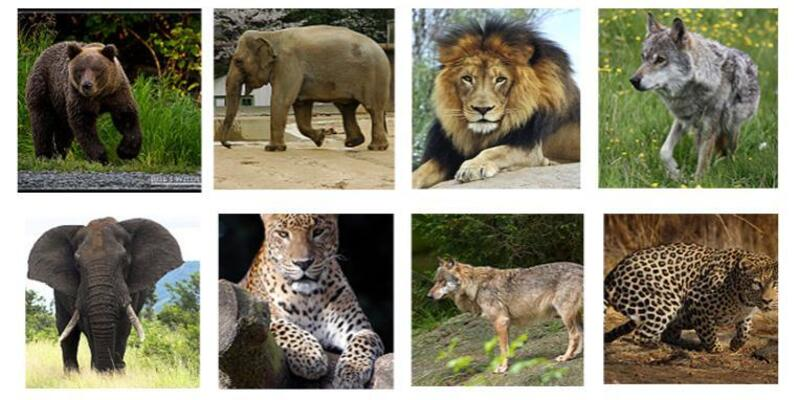
\includegraphics[width = 0.7\textwidth]{Figures/img/dataset-cover.png}
    \caption{Cover image of the animal-data\cite{animal-data} dataset on kaggle}
    \label{fig:label1}
\end{figure}